%% LyX 2.3.4.2 created this file.  For more info, see http://www.lyx.org/.
%% Do not edit unless you really know what you are doing.
\documentclass[english]{article}
\usepackage[T1]{fontenc}
\usepackage[latin9]{inputenc}
\usepackage{verbatim}
\usepackage{float}
\usepackage{graphicx}

\makeatletter

%%%%%%%%%%%%%%%%%%%%%%%%%%%%%% LyX specific LaTeX commands.
%% Because html converters don't know tabularnewline
\providecommand{\tabularnewline}{\\}
%% A simple dot to overcome graphicx limitations
\newcommand{\lyxdot}{.}


\makeatother

\usepackage{babel}
\begin{document}
\title{Prediction of Protein-Protein Interactions on the Human and Rice Interactome }
\author{Nicol�s Antonio L�pez Rozo}
\maketitle
\begin{abstract}

Previous Network-based efforts to predict unmapped protein-protein
interactions (PPI's) suggest that proteins with multiple paths of
length 3 (L3) are more likely to be connected. This paper extends
this so-called L3 principle by taking into account feature extraction
and using \texttt{XGBoost} techniques for prediction. In particular,
we train the model using handcrafted features as well as features
learned from embeddings using \texttt{Node2Vec}. Our main result shows
that while L3 remains an important principle for predicting links,
the approach is outperform by using embedded features. The mentioned
approaches are compared using the human and the rice interactomes.
\end{abstract}
\begin{comment}
need include a feature that compares the dimension of the embedding
is useful for prediction with L3 to show that they independent measures
- we do not want to be learning L3 through node2vec
\end{comment}


\section{Introduction}

\begin{comment}
Need to add other relevant references
\end{comment}

Proteins are the chief actors of biological functionality inside of
the cell, and as such, do not usually work as single substances but
rather as a part of dynamic networks, interacting with other substances
for a wide variety of purposes \cite{Lin2017}.

Protein-protein interactions (PPIs) have a key role in a variety of
biological processes such as signal transduction, homeostasis control,
stress responses, plant defense and organ formation. On the molecular
level, PPIs have importance in protein phosphorylation, transcriptional
co-factor recruitment, transporter activation and many others, thus
playing an essential role in many physiological and developmental
processes in virtually all organisms \cite{Zhang_2010_PPI}.

Prediction of potentially relevant, yet unexplored PPIs is a current
research topic on bioinformatics and therefore, several authors have
proposed different methods for extrapolating information from the
existing PPI networks. As presented by Kovacs et al (2019), information
related to counting paths of length 3 (L3) seems to outperform state-of-the-art
methods when it comes to predict interactions among proteins for a
variety of model organisms such as yeast (\emph{S. cerevisiae}), Arabidopsis
(\emph{A. thaliana}), worm (\emph{C. elegans}), fly (\emph{D. melanogaster}),
fission yeast (\emph{S. pombe}) and mouse (\emph{M. musculus}), as
well as on the human interactome \cite{Kovacs2019}.

The most common way to validate PPI's is the \emph{Yeast-Two-Hybrid}
technique (also known as \emph{two-hybrid screening} or \emph{Y2H}),
which is based on the expression of a specific reporter gene that
activates by the binding of a DNA-binding Domain (DB) and an Activation
Domain (AD) of a Transcription Factor that binds to an Upstream Activation
Sequence (UAS). For the Y2H technique, a protein is fused to the DB
domain (known as \emph{bait}) and another one to the AD (known as
\emph{prey}). If the proteins do not interact, then the reporter gene
is not expressed. Otherwise, the reporter gene expression is activated
by the activation domain.

\begin{comment}
NL: I will make this figure myself
\end{comment}

\begin{figure}[h]
\caption{Yeast-2-Hybrid Technique}

\noindent \centering{}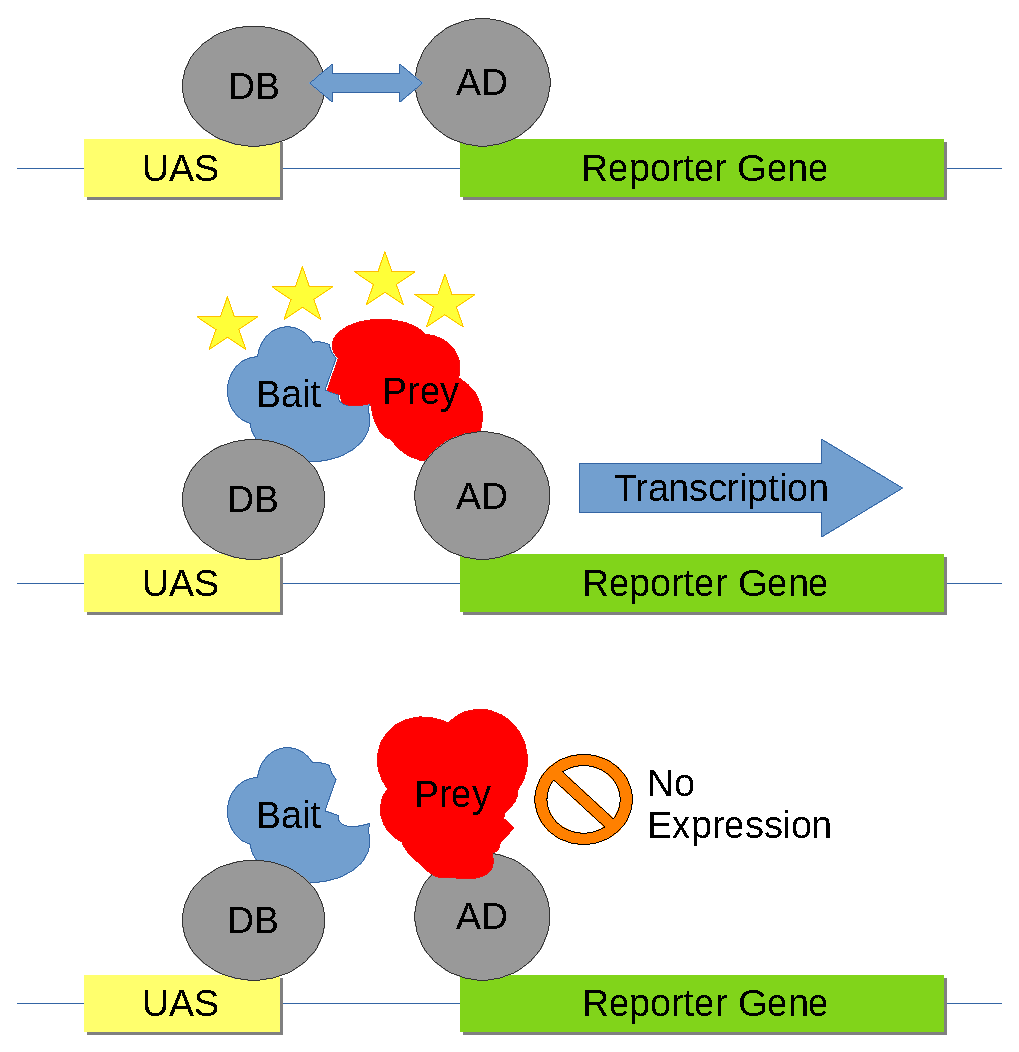
\includegraphics[width=1\columnwidth]{Y2H}
\end{figure}

Having several of these Y2H results allows scientists to establish
a PPI network, where all known interactions for each protein are represented.
Several algorithms are proposed over these networks in order to predict
unknown interactions. In this report, three prediction methods are
presented and their results are shown: Common Neighbors (\textbf{CN}),
which uses the length-2 path count; raw count of paths of length 3
(\textbf{A3}); and degree-normalized length-3 paths score (\textbf{L3}).

Focus of the present study is to evaluate different methods for predicting
protein-protein interactions (PPIs) using the existing knowledge of
the network, which is an undirected graph. The traditional way is
usually based on social networks analysis, more specifically on the
Triadic Closure Principle (TCP), that states that the more common
shared friends that two people have, the more likely that they know
each other. As shown by previous studies, the mentioned approach fails
because it does not consider the structural and chemical properties
of the proteins \cite{Kovacs2019}.

For achieving the described results, human and rice PPI networks are
used and compared using state-of-the-art methods, as well as the proposed
ones (CN, A3, L3). In the case of the human network, human interactome
(\emph{HI-II-14}), as well as a curated version of it (\emph{HI-TESTED})
were used. A massive experimental assay was carried on and its results
were consolidated and used to build a validation network (\emph{HI-III}). 

\section{Materials and Methods}

\subsection{Data Availability}

Human interactome data and base source code were downloaded from the
repository of the length-3 degree normalized paths methodology \cite{Kovacs2019}:
the dataset \emph{HI-II-14} and \emph{HI-TESTED} are used for prediction
and the dataset \emph{HI-III} is used for validation.

Rice interactome information was downloaded from the STRING database
\cite{Szklarczyk2019}, corresponding to the \emph{Oryza sativa} subspecies.
The downloaded file was \emph{4530.protein.links.detailed.v11.0.txt}.
and contains more than 8 million PPIs from several resources. For
the purpose of this study and based on previous work, only PPIs with
evidence from curated databases were used (i.e. rows where the column
\emph{databases} has a value greater than zero), resulting in a network
with $5025$ nodes and $164420$ edges.

\subsection{Code Implementation}

Previous code implementation was adapted from \texttt{C++} to \texttt{Python}
(V3.6), in order to unify the algorithms into one single script. For
the purpose of algorithmic validation, the three methods were implemented
from scratch with basic functionalities and data structures of the
\texttt{Python} language.

\subsection{Data Preprocessing}

Information for the human interactome was used as-is, which corresponds
to networks of $4298$, $3727$ and $5604$ proteins and $13868$,
$9433$ and $23322$ interactions.

For the rice interactome, an additional preprocessing was performed.
The filtered network for rice consists of $5025$ proteins (nodes)
and $164420$ interactions (edges) distributed among $178$ connected
components. The connected component with the greatest number of edges
was selected in this case. The extracted connected component consists
of $n=4390$ nodes and $m=163319$ edges, which corresponds to $99.33%\%
$ of filtered edges. Further investigation is applied to this network,
which is very similar in number of nodes to the curated information
on the human interactome, although rice network is much more connected.

\subsection{Edge Prediction}

For the interaction prediction for each network, the algorithms described
below were used. It is important to keep in mind how the protein-protein
interaction (PPI) network $G=(V,E)$ is conceptualized: each node
($v_{i}\in V$) represents a protein and each undirected edge ($e_{b}=\{v_{i},v_{j}\},\,e_{b}\in E$)
represents and interaction among proteins $v_{i}$ and $v_{j}$.
\begin{description}
\item [{Common~Neighbors~(CN)}] This method is based on the Triadic Closure
Principle: ``the more common friends two individuals have, the more
likely that they know each other''. For the implementation of this
method, $A{{}^2}$ matrix is calculated, being $A$ the adjacency
matrix of the network.
\item [{Length-3~Paths~(A3)}] This is the simplest implementation of
the proposed insight of ``if my friends and your friends interact,
then we might interact too''. The calculating is carried on with
$A{{}^3}$, i.e, the third power of the adjacency matrix.
\item [{Degree-normalized~L-3~Score~(L3)}] The previous approach might
overestimate the importance of some edges due to intermediate hubs
which add many shortcuts in the graph. To address that issue, a degree
normalization for the path $X\rightarrow U\rightarrow V\rightarrow Y$
is applied by considering the degree $k$ of the intermediate nodes
$U$ and $V$, as follows.
\[
p_{XY}=\sum_{U,V}\frac{A_{XU}\cdot A_{UV}\cdot A_{VY}}{\sqrt{k_{U}\cdot k_{V}}}
\]
\\
where $A_{ij}$ represents the value of the adjacency matrix for nodes
$i$ and $j$: 1 if the edge $\{i,j\}$ exists, 0 otherwise.
\end{description}

\subsection{Sampling Procedure}

For each network of protein interactions, the following procedure
was performed 10 times in order to address the stochastic nature of
the process and have a consensus:
\begin{itemize}
\item A percentage of interactions is removed at random from the network
(20\%).
\item The same amount of removed interactions are then predicted using the
main methods for prediction mentioned by Kovacs et al (2019): Common
Neighbors (\textbf{A2}), raw path count of paths of length 3 (\textbf{A3})
and the Length-3 degree-normalized score (\textbf{L3}).
\item A test dataset is created as follows: all removed edges are included
(as observed positives for the ML algorithm) and from the predicted
edges of \textbf{A2}, \textbf{A3} and \textbf{L3} that don't lie in
the previous classification (observed negatives), a random subset
is chosen such that the dataset is balanced, that is, the amount of
observed positive labels is equal to the observed negative labels.
\item Once the dataset is ready, it is randomly partitioned: 80\% is used
for \texttt{XGBoost} model training and 20\% is used for validation.
It is important to have in mind that balanced distribution of the
positive and negative labels in the datasets was satisfied.
\end{itemize}

\subsection{Feature Extraction with \texttt{Node2Vec}}

The \texttt{Node2Vec} module was used for extracting features of the
rice interactome graph. The parameters and considerations for the
model were:
\begin{itemize}
\item All paths in the random walks are equally likely (\texttt{p=1, q=1})
\item Use a modest number of dimensions and threads for calculation (\texttt{dimensions=16,
workers=4})
\item Since length-3 paths are the defining property in this study, there
is no necessity for longer walks. However, it is important to try
out many possible redundant routes and to consider a window of at
least 4 (\texttt{walk\_length=5, num\_walks=300, window=5})
\item Other standard parameters were left with default values (\texttt{min\_count=1,
batch\_words=4})
\item Edge embeddings were calculated using a geometric ratio of the node
embeddings (\texttt{HadamardEmbedder})
\end{itemize}

\subsection{Handcrafted Feature}

Due to the poor results of the \emph{raw} Length-3 counting (\textbf{A3}),
a different approach for this information was carried out in the present
study: As it still gives a lot of information that might be useful
for a predictive routine, this counting was normalized (dividing by
the greatest counting in the \textbf{A3} top predictions) and then
used as a feature for the Machine Learning algorithm. For completeness,
also \textbf{CN} and \textbf{L3} information was used as a possible
feature. Finally, the case were no handcrafted feature was also considered,
that is, only the features extracted from the structure of the network.

\subsection{Feature to Predict: Existence}

The feature to predict corresponds to the possible existence (\emph{True/False})
of a link based on the existing information of the network, using
the network itself in a random sub\_exploration (\texttt{Node2Vec})
as well as in a structured search (A3). This property is evaluated
by taking out a fraction of the edges and then trying to predict for
a given set of possible edges if they have a high probability to belong
to the original network.

\subsection{Machine Learning Algorithm}

The Extreme Gradient Boosting implementation of gradient boosted trees
is applied in this study to evaluate the existence of an edge. Gradient
boosted trees are usually used for supervised learning problems, where
the training data $X_{i}$ has multiple features and pretends to explain
(or predict) a target variable $Y_{i}$. The corresponding implementation
applied for this study is \texttt{XGBoost}, available publicly.

The selected parameters for the model were:\texttt{ max\_depth=3},
\texttt{colsample\_bytree=0.6} and \texttt{eval\_metric=''auc''}.

\subsection{Result Validation}

As mentioned before, 80\% of the final dataset was randomly selected
and used for training, while the remaining 20\% was used for validation.
The whole training-validation procedure was applied 10 times.

The chosen metric for validation was the Area under the Curve (\textbf{AUC})
of the Receiver Operating Characteristic (\textbf{ROC}). This curve
corresponds to plot the sensitivity (probability of predicting a real
positive as positive) against 1-specificity (probability of predicting
a real negative as positive). It is worth to remind that AUC values
move in the range $[0,1]$, where 1 is a perfect prediction and 0.5
corresponds to a random guess. Normally, values over 0.8 of AUC are
considered good.

\section{Results and Discussion}

\subsection{Rice Interactome}

For the rice interactome, the different model-features combinations
were trained and validated. After executing the mentioned routines,
the results are shown in Figure \ref{F1}. First, one should have
a baseline of comparison, which in this case corresponds to \texttt{Node2Vec}
without any additional feature included. The plot below shows those
results, and one can see that its mean performance using the AUC metric
is 0.52, and that the results among the 10 repetitions are consistent.
This results mean that the model using only the default features perform
barely as good as a random choice of the labels.

\begin{figure}[H]
\noindent \begin{centering}
\caption{\label{F1}Summary ROC curves for \texttt{Node2Vec} model alone}
\par\end{centering}
\noindent \raggedleft{}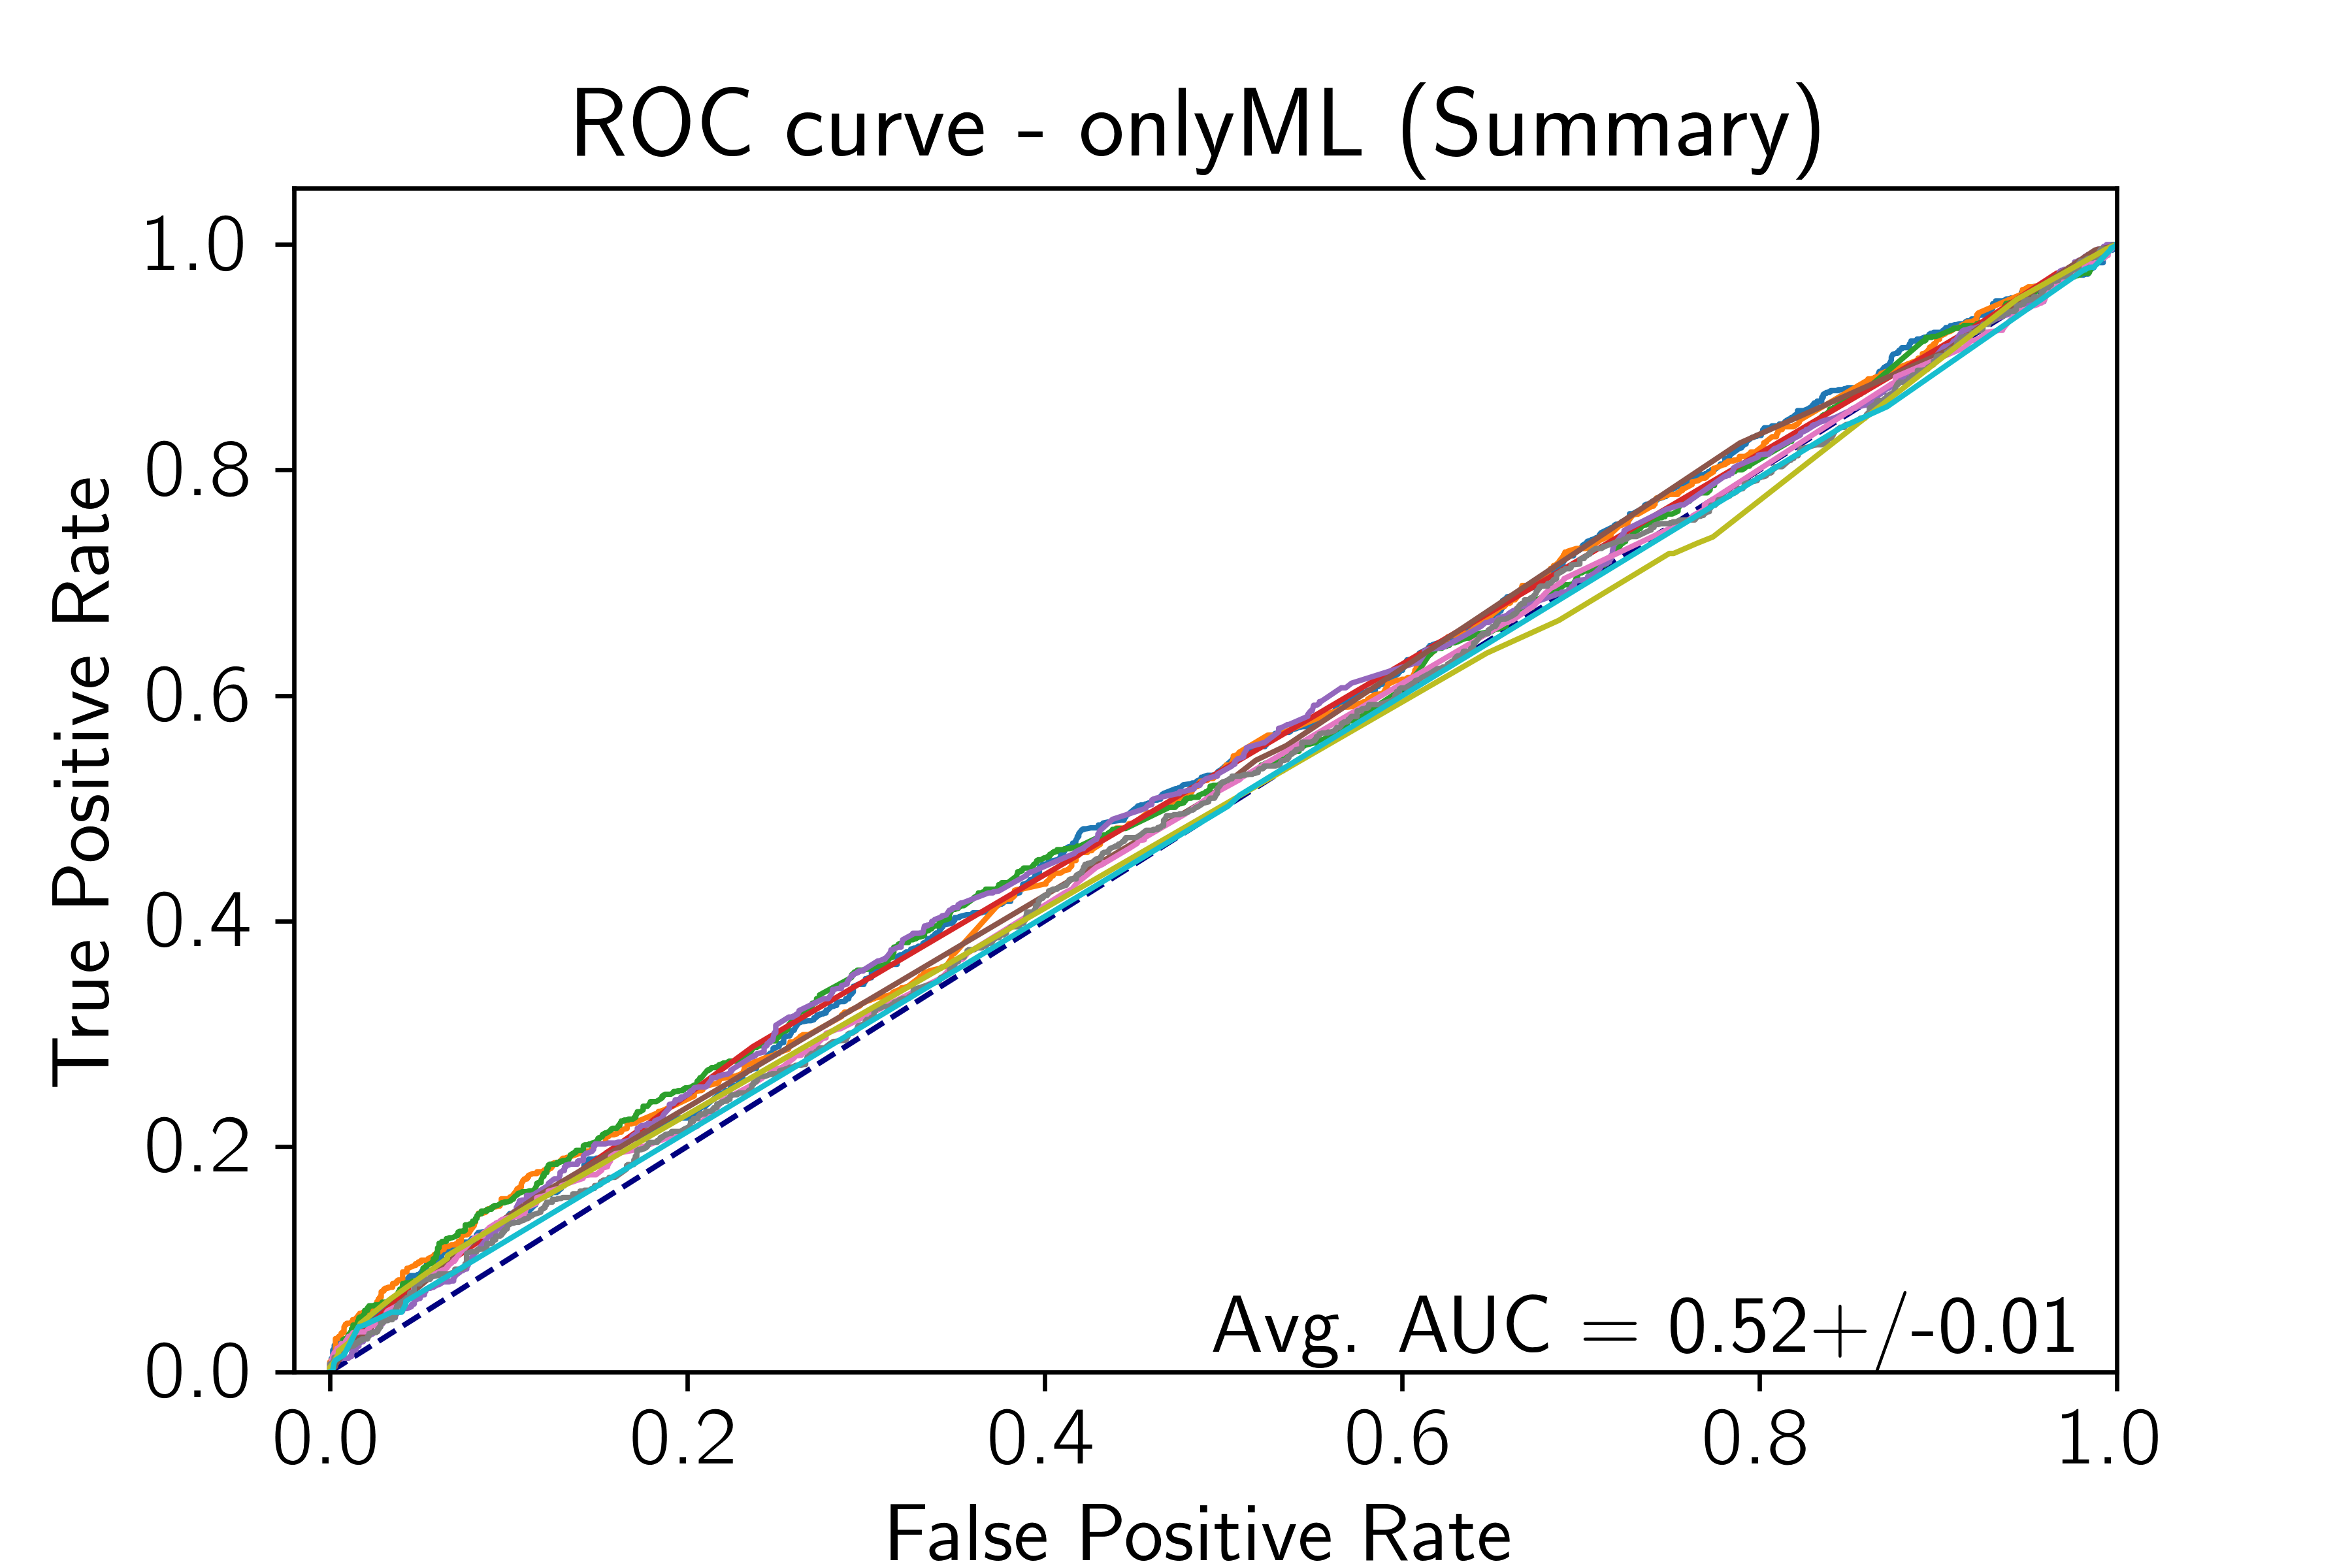
\includegraphics[width=0.95\columnwidth]{Only_ML/ROConlyML_SUMMARY}
\end{figure}


\section{(PENDING FROM HERE ON)}

\begin{figure}[h]
\caption{Methods Comparison for \emph{HI-II-14}}

\noindent \centering{}\includegraphics[width=1\columnwidth]{\string"/home/ocin/Documents/02 Asignaturas/10 GraphAnalytics/Project1/hi-ii-14.txt\string".eps}
\end{figure}

\begin{figure}[h]
\caption{Methods Comparison for \emph{HI-TESTED}}

\noindent \centering{}\includegraphics[width=1\columnwidth]{\string"/home/ocin/Documents/02 Asignaturas/10 GraphAnalytics/Project1/hi-tested.txt\string".eps}
\end{figure}

As it can be inferred from the plots, L3-based predictions outperform
their $A{{}^2}$ counterparts. Results also show that L3-score and
$A^{3}$predictions follow a very similar trend. 

When analyzing the robustness of each of the networks, the following
values for the Weighted Spectral Distribution were found. For a robustness
reference, the Erdos-Renyi model was used to generate a random network
with the same number of nodes and edges and on those random networks,
the WSD was measured.
\begin{center}
\begin{table}[H]
\caption{Validation of Weighted Spectral Distribution}

\centering{}%
\begin{tabular}{|c|c|c|}
\hline 
Network & Network WSD & Erdos-Renyi WSD\tabularnewline
\hline 
\hline 
HI-II-14 & 393.4939 & 198.7706\tabularnewline
\hline 
HI-TESTED & 423.3902 & 276.1065\tabularnewline
\hline 
HI-III (VALID.) & 373.9369 & 153.5329\tabularnewline
\hline 
\end{tabular}
\end{table}
\par\end{center}

The table shows that the three networks used in this report are robust,
because the are significantly more robust than a network with the
same density generated randomly.

\section{Conclusions}

Taking into account the different results validated in this report,
one can conclude that length-3 path methodologies might work better
on protein-protein interactions than its traditional length-2 (TCP
based) counterparts. On the other hand, it can be seen that degree-normalization
has little effect on the predictions, i.e., non-normalized $A{{}^3}$
matrix predictions are still a good methodology for edge prediction
on PPI networks.

Previous result comes as no surprise when the biological basis of
protein interactions is considered: It is necessary that protein A
and protein B have complementary structures in order to interact,
and when classical paths of length 2 are used, the predicted protein
interactions usually have the same structures, and not complementary
ones.

\begin{comment}
please update the conclusions - WSD does not seem relevant
\end{comment}

For the analyzed networks, it is also important to highlight their
robustness when compared to a random network with the same density:
if weighted spectral distribution (WSD) is used, then the used networks
are on average twice as robust as their random network versions.

\bibliographystyle{plain}
\bibliography{refs}

\end{document}
